\begin{center}
\Huge
Enhedscirklen og trigonometriske funktioner
\end{center}

\section*{Enhedscirklen}
\stepcounter{section}

Vi har tidligere arbejdet med de trigonometriske funktioner $\cos$, $\sin$ og $\tan$, og vi skal nu bruge \textit{enhedscirklen} til at definere dem. Enhedscirklen kan ses på Figur \ref{fig:enhed}
\begin{figure}[H]
	\begin{center}
	\begin{tikzpicture}
		\begin{axis}[
			axis lines = center, 
			xmin = -1.4, xmax = 1.4, 
			ymin = -1.4, ymax = 1.4, 
			x = 4cm, y = 4cm,
			minor xtick = {-1.4,-1.2,...,1.2,1.4},
			minor ytick = {-1.4,-1.2,...,1.2,1.4},
			xtick = {-1.6},
			ytick = {-1.6},
			xlabel = $x$, ylabel = $y$
		]
			%Shifted tick labels since unit circle would otherwise be in the way:
			\node[xshift = 5pt, yshift = -10pt] at (axis cs:1,0) {1};
			\node[xshift = -8pt, yshift = 5pt] at (axis cs:0,1) {1};
			%Circle, lines and angle:
			\draw[color = teal, thick] (axis cs:0,0) circle (4cm);
			\draw[thick, color = teal] (axis cs: 0,0) to (axis cs: {cos(45)},{sin(45)});
			\draw[thick, color = teal] (axis cs: 0.2,0) arc (0:45:0.8cm) node[midway, xshift = 5pt, yshift = 2pt] {$v$};
			\draw[dashed, thick, color = teal] (axis cs: {cos(45)},{sin(45)}) to (axis cs: {cos(45)},0);
			\draw[dashed, thick, color = teal] (axis cs: {cos(45)},{sin(45)}) to (axis cs: 0,{sin(45)});
			%Text:
			\node[color = teal, anchor = east, xshift = -2pt] at (axis cs: 0,{sin(45)}) {$\sin(v)$};
			\node[color = teal, anchor = north, yshift = -2pt] at (axis cs: {cos(45)},0 ) {$\cos(v)$};
			\node[color = teal, anchor = south west] at (axis cs: {cos(45)},{sin(45)}) {$P_v$};

		\end{axis}
	\end{tikzpicture}
	\end{center}
	\caption{Definition af $\cos$ og $\sin$ ud fra enhedscirklen}
	\label{fig:enhed}
\end{figure}
Enhedscirklen er en cirkel med centrum i origo og radius $1$. Vi kan bruge enhedscirklen til at definere $\cos$ og $\sin$.
\begin{defn}
Lad $P_v$ være et punkt på enhedscirklen, så vinklen mellem stedvektoren $\vv{OP_v}$ og $x$-aksen er $v$. Så defineres funktionerne $\cos(v)$ og $\sin(v)$ som koordinaterne til $P_v$:
\begin{align*}
P_v = (\cos(v),\sin(v)).
\end{align*}
\end{defn}

\begin{exa}
Det gælder, at $\cos(0) = 1$ og $\sin(0)=0$, da koordinatsættet til $P_0$ er 
\begin{align*}
P_0 = (1,0) = (\cos(0),\sin(0)).
\end{align*}
\end{exa}

Skal vi anvende de trigonometriske funktioner i Maple og vi ønsker at anvende grader, så skal vi skrive
\begin{align*}
	&\texttt{with(Gym):} \\
	&\texttt{Cos(v)} \\	
	&\texttt{Sin(v)}
\end{align*}



Tangens er den sidste trigonometriske funktion, vi skal betragte. Denne er defineret som 
\begin{align*}
\tan(v) = \frac{\sin(v)}{\cos(v)}.
\end{align*}


\section*{Retvinklede trekanter}
\stepcounter{section}

\begin{setn}
	\label{setn:trigretvinkel}
Lad $ABC$ være en trekant med punkterne $A$,  $B$ og $C$ som hjørner, og lad $C$ være en ret vinkel. Så gælder der for vinklen $v$, der er vinklen i enten hjørnet $A$ eller $B$, at 
\begin{align*}
\cos(v) &= \frac{\textnormal{hosliggende katete}}{\textnormal{hypotenuse}}\\
\sin(v) &= \frac{\textnormal{modstående katete}}{\textnormal{hypotenuse}}\\
\tan(v) &= \frac{\textnormal{modstående katete}}{\textnormal{hosliggende katete}}
\end{align*}
\end{setn}
\begin{proof}
Bevises som opgave.
\end{proof}


\subsection*{Opgave 1}
\begin{center}
	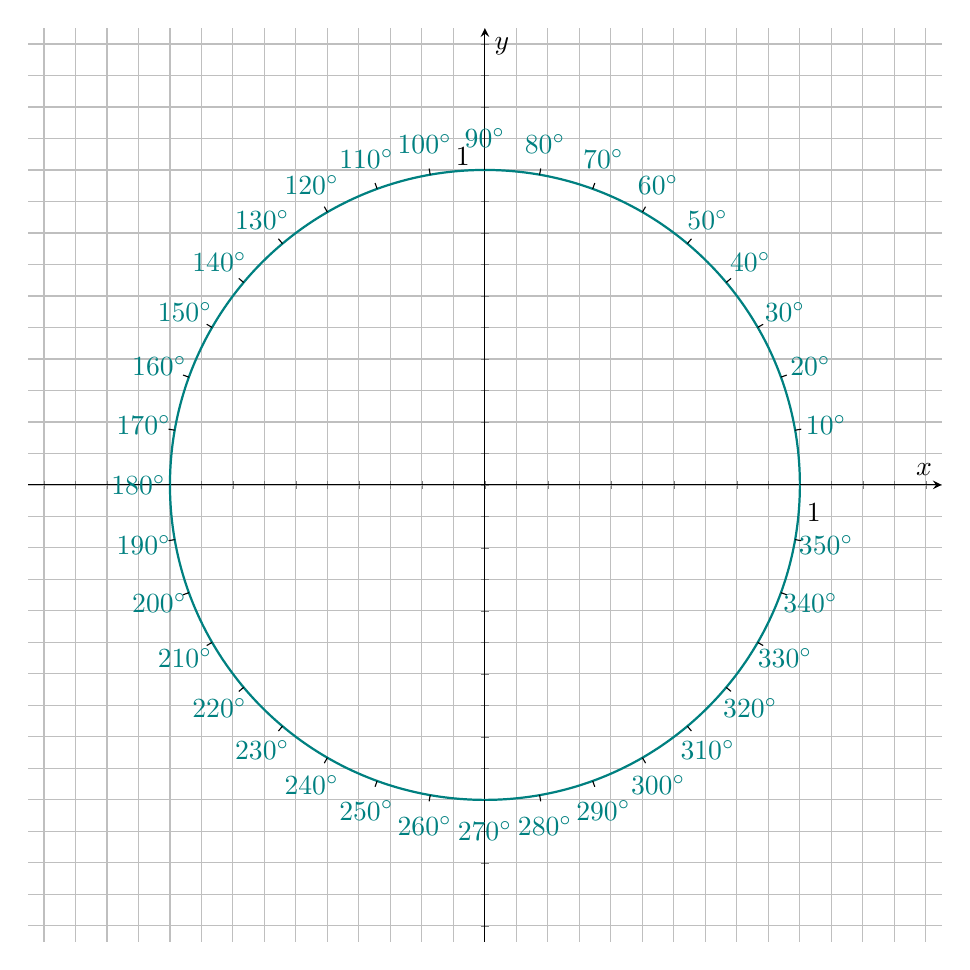
\begin{tikzpicture}
		\begin{axis}[
			axis lines = center, 
			xmin = -1.45, xmax = 1.45, 
			ymin = -1.45, ymax = 1.45, 
			x = 4cm, y = 4cm,
			minor xtick = {-1.4,-1.3,...,1.3,1.4},
			minor ytick = {-1.4,-1.3,...,1.3,1.4},
			grid = both,
			xtick = {-1.6},
			ytick = {-1.6},
			xlabel = $x$, ylabel = $y$
		]
			%Shifted tick labels since unit circle would otherwise be in the way:
			\node[xshift = 5pt, yshift = -10pt] at (axis cs:1,0) {1};
			\node[xshift = -8pt, yshift = 5pt] at (axis cs:0,1) {1};
			\draw[color = teal, thick] (axis cs:0,0) circle (4cm);
			%Ticks on circle 
			\pgfplotsinvokeforeach{0,1,...,35}
			{
				\draw (axis cs: {cos(#1*10)},{sin(#1*10)})-- (axis cs: {1.02*cos(#1*10)},{1.02*sin(#1*10)});
			}
			\pgfplotsinvokeforeach{10,20,...,350}
			{
				\node[color = teal] at (axis cs: {1.10*cos(#1)},{1.10*sin(#1)}) {$#1^\circ$};
			}
		\end{axis}
	\end{tikzpicture}
	\end{center}
Brug enhedscirklen til at aflæse $\cos(v)$ og $\sin(v)$ for følgende vinkler. (Det behøver ikke være helt præcist.) 
\begin{center}
	\begin{tabular}{c|c|c|c|c|c|c}
		$v$ & 90 & 70 & 120 & 190 & 350 & 45 \\
		\hline
		$\cos(v)$ & 0 & & & & & \\
		\hline
		$\sin(v)$ & 1 & & & & & 
	\end{tabular}	
\end{center}

\newpage
\subsection*{Opgave 2}

Brug hvad du ved om ensvinklede trekanter til at bestemme sidelængderne $a$ og $b$ i følgende trekant:

\begin{center}
	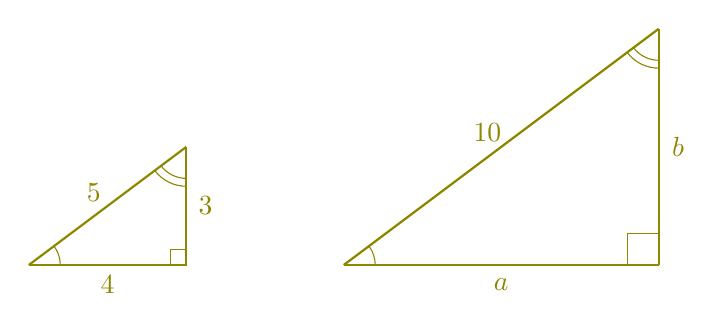
\begin{tikzpicture}
		\draw[color = olive, thick] (-2,0) -- (0,0) node[midway, yshift = -7pt] {4};
		\draw[color = olive, thick] (0,0) -- (0,1.5) node[midway, xshift = 7pt] {3};
		\draw[color = olive, thick] (-2,0) -- (0,1.5) node[midway, yshift = 5pt, xshift = -5pt] {5};
		\draw[color = olive] (0,0) rectangle (-0.2,0.2);
		\draw[color = olive, thick] (2,0) -- (6,0) node[midway, yshift = -7pt] {$a$};
		\draw[color = olive, thick] (6,3) -- (6,0) node[midway, xshift = 7pt] {$b$};
		\draw[color = olive, thick] (2,0) -- (6,3) node[midway, yshift = 5pt,
		xshift = -5pt] {10};
		\draw[color = olive] (6,0) rectangle (5.6,0.4);
		%angle arcs for first triangle
		\draw[color = olive] (-2+.4,0) arc (0:{acos(4/5)}:0.4);
		\draw[color = olive] (0,1.5-0.4) arc (-90:-{acos(3/5)}-90:0.4);
		\draw[color = olive] (0,1.5-0.5) arc (-90:-{acos(3/5)}-90:0.5);
		%angle arcs for second triangle
		\draw[color = olive] (2+.4,0) arc (0:{acos(4/5)}:0.4);
		\draw[color = olive] (6,3-0.4) arc (-90:-{acos(3/5)}-90:0.4);
		\draw[color = olive] (6,3-0.5) arc (-90:-{acos(3/5)}-90:0.5);
	\end{tikzpicture}
\end{center}

\newpage
\subsection*{Opgave 3}
Vi skal nu bevise Sætning \ref{setn:trigretvinkel}. Vi betragter derfor Figur \ref{fig:bevis}

\begin{figure}[H]
	\begin{center}
	\begin{tikzpicture}
		\begin{axis}[
			axis lines = center, 
			xmin = -1.4, xmax = 3.4, 
			ymin = -1.4, ymax = 3.4, 
			x = 3cm, y = 3cm,
			xtick = {-1.6},
			ytick = {-1.6},
			xlabel = $x$, ylabel = $y$
		]
			%Shifted tick labels since unit circle would otherwise be in the way:
			\node[xshift = 5pt, yshift = -10pt] at (axis cs:1,0) {1};
			\node[xshift = -8pt, yshift = 5pt] at (axis cs:0,1) {1};
			%Circle, lines and angle:
			\draw[color = teal, thick] (axis cs:0,0) circle (3cm);
			\draw[thick, color = teal] (axis cs: 0,0) to (axis cs: {cos(45)},{sin(45)});
			\draw[thick, color = teal] (axis cs: 0.2,0) arc (0:45:0.6cm) node[midway, xshift = 5pt, yshift = 2pt] {$v$};
			\draw[thick, color = teal] (axis cs: {cos(45)},{sin(45)}) to (axis cs: {cos(45)},0);
			\draw[thick, color = teal] (axis cs: 0,0) to (axis cs: {cos(45)},0);
			\draw[color = teal, thick] (axis cs: {cos(45)},0) rectangle (axis cs: {cos(45)-0.1},0.1);
			\draw[color = teal, thick] (axis cs: 0,0) -- (axis cs: 3,0)
			node[midway, yshift = -7pt] {$a$};
			\draw[color = teal, thick] (axis cs: 3,0) -- (axis cs: 3,3) node[midway, xshift = 7pt] {$b$};
			\draw[color = teal, thick] (axis cs: 0,0) -- (axis cs: 3,3) node[midway, yshift = 7pt, xshift = -5pt] {$c$};
			\draw[color = teal, thick] (axis cs: 3,0) rectangle (axis cs: 3-0.1,0.1);
		\end{axis}
	\end{tikzpicture}
	\end{center}
	\caption{To ensvinklede trekanter i et koordinatsystem med enhedscirklen}
	\label{fig:bevis}
\end{figure}

\begin{enumerate}[label=\roman*)]
	\item Tegn Figur \ref{fig:bevis} i jeres gruppe. 
	\item Hvad er længden af hypotenusen for den lille trekant? Skriv det på jeres figur.
	\item Hvad er højden og bredden af den lille trekant? Sammenlign eventuelt med enhedscirklen på Figur \ref{fig:enhed} eller tænkt på Opgave 1. 
	\item Hvor mange gange større er den store trekant end den lille trekant? Tænk på hvad i gjorde i Opgave 2 (I skal ikke måle, men regne med bogstaver).
	\item Hvad skal vi gange bredden med i den lille trekant for at få $a$? Skriv det udtryk op.
	\item Hvad skal vi gange højden med i den lille trekant for at få $b$? Skriv det udtryk op.
	\item Isolér $\cos(v)$ i det første udtryk. 
	\item Isolér $\sin(v)$ i det andet udtryk. 
	\item Hvad er hyp, hos og mod i den store trekant? Indsæt det i de to udtryk. 
	\item Sammenlign jeres resultat med Sætning \ref{setn:trigretvinkel}.
	\item Indsæt jeres udtryk for $\cos(v)$ og $\sin(v)$ i udtrykket
	\begin{align*}
		\tan(v) = \frac{\sin(v)}{\cos(v)}.	
	\end{align*}	 
	\item Brug brøkregneregler til at forkorte udtrykket og sammenlign herefter med Sætning \ref{setn:trigretvinkel}.
\end{enumerate}
